\section{Билет 13. Метод Фурье решения смешанной задачи для уравнения колебаний струны с закреплёнными концами. Обоснование метода для случая однородного уравнения.}
% Набрано Шлёнским Владиславом
\subsection{Формулировка задачи}
\textbf{Задача:}
\begin{equation}
\label{eq:13_1}
\begin{cases}
	u_{tt} - a^2u_{xx} = f(x, t),\; (t, x) \in Q_{T} = (0, T) \times (0, l), \\
    u\bigr|_{t = 0} = u_{0}(x);\; u_{t}\bigr|_{t =0} = u_{1}(x),\; x \in [0, l], \\
    u\bigr|_{x = 0} = \psi_{0}(t),\; u\bigr|_{x = l} = \psi_{1}(t);\; t \in [0, T].
\end{cases}
\end{equation}
Рассматриваем её \textit{классическое решение} - функцию $u(t, x) \in C^{2}\bigl(Q_{T}\bigr) \cap C^{1}\bigl(\overline{Q}_{T}\bigr)$, удовлетворяющую уравнению, начальным и граничным условиям. \\
\subsection{Теорема единственности}
\begin{theorem}[Единственности]
Не может существовать более одного классического решения задачи ~\ref{eq:13_1}.
\end{theorem}
\begin{proof}
\paragraph{Единственность решения.}
Для двух решений $\tilde{u}_{1}$ и $\tilde{u}_{2}$  построим $V(t, x) = \tilde{u}_{1} - \tilde{u}_{2} \in C^{2}\bigl(Q_{T}\bigr) \cap C^{1}\bigl(\overline{Q}_{T}\bigr)$.\\$V$ - решение полностью однородной задачи:
\begin{equation*}
\begin{cases}
V_{tt} - a^2V_{xx} = 0, \\
V\bigr|_{t = 0} = V_t\bigr|_{t = 0} = 0, \\
V\bigr|_{x = 0} = V\bigr|_{x = l} = 0.
\end{cases}
\end{equation*}
Докажем, что $V \equiv 0$ с помощью интеграла энергии: рассмотрим функцию $I = V_{t}\bigl[V_{tt} - a^2V_{xx}\bigr],\; (t, x) \in Q_{T}$.
\begin{equation*}
I = V_{t}V_{tt} - a^2V_{t}V_{xx} = \dfrac{1}{2}\bigl(V_{t}^{2}\bigr)_{t} - a^2\bigl(V_{t}V_{x}
\bigr)_{x} + a^2\underbrace{V_{x}V_{xt}}_{\frac{1}{2} \bigl(V_{x}^{2}\bigr)_{t}} = \underbrace{\biggl(\dfrac{V_{t}^2 + a^2V_{x}^{2}}{2}\biggr)_{t}}_{F^1_t}  \underbrace{ - \bigl(a^{2}V_{t}V_{x}\bigr)_{x}}_{F_{x}^{2}}\; \biggr|\; \div\vec{F} = \div \begin{pmatrix}
F^1 \\
F^2
\end{pmatrix}
\end{equation*}
Воспользуемся формулой Грина: $\iint\limits_{\Omega}\bigl(\dfrac{\partial Q}{\partial x} - \dfrac{\partial P}{\partial y}\bigr)\;dxdy = \oint\limits_{\partial \Omega}Q\;dy + P\;dx$.
Для её использования требуется непрерывность производных до границы, поэтому напишем её для области: $Q_{\tau, \varepsilon} = \{(t, x)\colon\; \varepsilon < t < \tau,\; \varepsilon < x < l - \varepsilon\}$.\\
\ \\
\begin{minipage}[c]{0.2\textwidth}
\begin{center}
\begin{tikzpicture}[scale=0.55]
  \tikzstyle{axes}=[]
  \tikzstyle{important line}=[very thick]
  \tikzstyle{information text}=[rounded corners,fill=red!10,inner sep=1ex]

   \begin{scope}[style=axes]
    \draw[->] (-0.2,0) -- (5,0) node[right] {$x$};
    \draw[->] (0,-0.2) -- (0,4) node[left] {$t$};
    \end{scope}

    \coordinate [label = {below: $\varepsilon$}] (A) at (0.5, 0);
    \coordinate [label = {left: $\varepsilon$}] (B) at (0, 0.5);
    \coordinate (C) at (0.5, 0.5);

    \draw [dashed] (A) -- (C) -- (B);

    \coordinate [label = {below: $l-\varepsilon$}] (D) at (3, 0);
    \coordinate (D1) at (3, 0.5);

    \draw [dashed] (D) -- (D1);

    \coordinate (Q) at (0.5, 2.5);
    \coordinate [label = {left: $\tau$}] (Q2) at (0, 2.5);
    \coordinate (Q1) at (3, 2.5);

    \coordinate [label = {below: $l$}] (E) at (4, 0);
    \coordinate [label = {left: $T$}] (F) at (0, 3);
    \coordinate (G) at (4, 3);
    \draw [dashed] (E) -- (G) -- (F);

    \draw [pattern = north east lines, pattern color = blue] (C) -- (D1) -- (Q1) -- (Q) -- cycle;
    \draw [dashed] (Q2) -- (Q); 
    
      \coordinate [label = {below:  \textbf{\LARGE $Q_{\tau, \varepsilon}$}}] (L) at (1.75, 1.95);
\end{tikzpicture}
%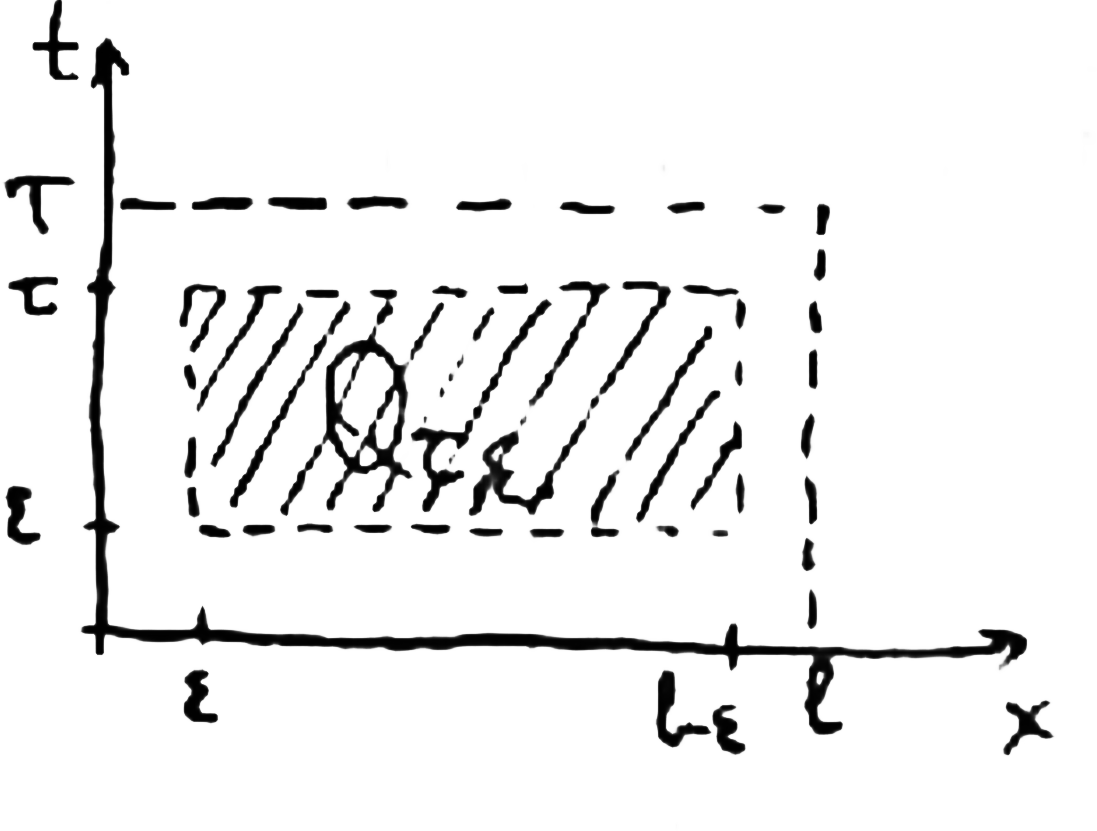
\includegraphics[scale = 0.2]{13_1_new}
\end{center}
\end{minipage}
\begin{minipage}[c]{0.8\textwidth}
$$0 = \iint\limits_{Q_{ \tau, \varepsilon}}I\;dxdt = \iint\limits_{Q_{\tau, \varepsilon}}\div \vec{F}\;dxdt = \oint\limits_{\partial Q_{\tau, \varepsilon}} \bfbr{-\dfrac{V_t^2 + a^2V_{x}^2}{2}\;dx - a^2V_tV_x\;dt}$$
\begin{center}
Распишем интеграл по $\partial Q_{\tau, \varepsilon}$:
\end{center}
\end{minipage}
\begin{equation*}
\int\limits_{\varepsilon}^{l - \varepsilon} \biggl( \dfrac{V_t^2 + a^2V_x^2}{2}\biggr)\biggr|_{t = \tau}\;dx - \int\limits_{\varepsilon}^{l - \varepsilon} \biggl( \dfrac{V_t^2 + a^2V_x^2}{2}\biggr)\biggr|_{t = \varepsilon}\;dx - \int\limits_{\varepsilon}^{\tau}\bigl(a^2V_xV_t\bigr)|_{x = l - \varepsilon}\;dt + \int\limits_{\varepsilon}^{\tau}\bigl(a^2V_xV_t\bigr)|_{x = \varepsilon}\;dt = 0
\end{equation*}
В пределе при $\varepsilon \to 0$ получаем :
\begin{align*}
 \because V_t(\varepsilon, x) \to V_t(0, x) = 0\; \; \; \; \; \; \; \because V_x(\varepsilon, x) \to V_x(0, x) = \dfrac{d}{dx}\bigl(V\bigr|_{t = 0} \bigr) = 0 \; \; \; \; \; \; \; \because \int_{\varepsilon}^{l-\varepsilon} \to \int_{0}^{l} {\tiny \text{(по определению несобственного интеграла)}} \\
\because \lim_{\varepsilon \rightarrow +0} V_t(t, l - \varepsilon) = V_t(t, l) = 0 \Rightarrow \cancelto{0}{\int\limits_0^\tau \bigl(a^2V_tV_x\bigr)\;dt}\; \;  \because \int\limits_{\varepsilon}^{l - \varepsilon}\brbr{\dfrac{V_t^2 + a^2V_x^2}{2}}\bigr|_{\tau = l}\; dx = \cancelto{0}{\int\limits_{0}^l \dfrac{V_t^2(0, x) + a^2V_x^2(0, x)}{2}\;dx\;\;\;\;\;\;}
\end{align*}
Аналогично для $\int\limits_{\varepsilon}^{\tau}(a^2V_tV_x)\bigr|_{x = \varepsilon}\;dt = 0$. Поэтому получаем, что: 
$$\int\limits_{0}^l \dfrac{V_t^2(\tau, x) + a^2V_x^2(\tau, x)}{2}\;dx = 0$$
Тогда $V_t^2(\tau, x) + a^2V_x(\tau, x) = 0 \Forall (x, t) \in (0, l) \times \tau$. \\
В любой точке $(t, x) \in Q_{\tau}\colon\; \vec{\nabla}V(t, x) = \vec{0} \Rightarrow V = \text{const}\Forall(t, x) \in Q_{\tau}$. \\
На замыкании в силу непрерывности $V$ в $\overline{Q}_{\tau}$ также будет $V \equiv \text{const}$, но на границе $V = 0 \Rightarrow V \equiv 0 \Forall (t, x) \in \overline{Q}_{\tau}$, поэтому \textbf{$\tilde{u}_{1} = \tilde{u}_{2}$}.
\paragraph{Существование решения} Будем рассматривать смешанную задачу для однородного уравнения колебаний струны при закреплённых концах.
\begin{equation*}
\label{eq:13_2}
\begin{cases}
	u_{tt} = a^2u_{xx},\; (t, x) \in Q_{\tau}, \\
	u\bigr|_{t = 0} = u_0(x),\; u_t\bigr|_{t = 0} = u_1(x),\; x \in [0, l], \\
	u\bigr|_{x = 0} = u\bigr|_{x = l} = 0,\; t \in [0, \tau].
\end{cases}
\end{equation*}
Рассмотрим дифференциальный оператор $-\Delta_{0}$:
$$\mathcal{D}(-\Delta) =\{X(x) \in C^2[0, l]\colon\; X(0) = X(l) = 0\}$$
У это оператора есть счётное однопараметрическое семейство собственных функий: $\lambda_k = \brbr{\dfrac{\pi k}{l}},\; X_k = sin(\lambda_k x),\; k \in \mathbb{N}$. \\
Решение будем искать в виде ряда $u(t, x) = \sum\limits_{k = 1}^{\infty} \Theta_k(t)X_k(x)$. Будем требовать выполнения следующих условий:
\begin{equation}
\begin{cases}
	u_0(x) \in C^3[0, l],\; u_1(x) \in C^2[0, l] - \textbf{условия гладкости}\\
	u_0(0) = u_0(l) = 0 - \text{для непрерывности решения на}\; \overline{Q}_{\tau}, \\
	u_1(0) = u_1(l) = 0 - \text{для принадлежности решения}\; C^1(\overline{Q}_{\tau}), \\
	u^{''}_0(0) = u_0(l)^{''} = 0 - \text{для принадлежности}\; C^2(\overline{Q}_{\tau}).
\end{cases}
\end{equation}

\textit{Последние три условия называются \textbf{условиями согласования}}. \\
Рассматриваемый оператор симметричен относительно скалярного произведения в $\mathbb{L}_2$, значит, собственные функции ортогональны в $\mathbb{L}_2$. Разложим $u_0, u_1$ в ряды Фурье по $X_k$ на $[0, l]$:
\begin{align*}
	u_0(x) = \sum\limits_{k = 1}^{\infty} A_kX_k,\; A_k = \dfrac{2}{l} \int\limits_{0}^l u_0(x)X_k\;dx \\
	u_1(x) = \sum\limits_{k = 1}^{\infty} B_kX_k,\; B_k = \dfrac{2}{l} \int\limits_{0}^l u_1(x)X_k\;dx 
\end{align*}
Формально подставляем в уравнение: $\sum\limits_{k = 1}^{\infty}\bfbr{\Theta^{\cdotp \cdotp}_k + a^2 \lambda_k^2\Theta_k}X_k = 0$. Из начальных условий: $\Theta_k(0) = A_k,\; \Theta^{\cdotp}_k(0) = B_k$. \\
В силу ортогональности $\{X_k(x)\}_{k = 1}^{\infty}$ получаем счётное число задач Коши:
\begin{equation*}
\begin{cases}
	\Theta^{\cdotp \cdotp}_k + a^2 \lambda_k^2\Theta_k = 0, \\
	\Theta_k(0) = A_k,\; \Theta^{\cdotp}_k(0) = B_k.
\end{cases}
\end{equation*}
Решение: $\Theta_k(t) = A_k\cos \brbr{\frac{a \pi k}{l}}t + \frac{l}{a \pi k}B_k \sin \brbr{\frac{a \pi k}{l}}t,\; t \in [0, \tau]$. 
\end{proof}
\subsection{Обоснование метода}
\begin{theorem}
Пусть данные Коши $u_0(x)$ и $u_1(x)$ удовлетворяют условиям гладкости и согласования. Тогда ряд $\sum\limits_{k = 1}^{\infty}\Theta_k(t)X_k(x)$ сходится абсолютно и равномерно в $\overline{Q}_{\tau}$. Его сумма принадлежит классу $C^2(\overline{Q}_{\tau})$ и является классическим решением задачи ~\ref{eq:13_2}. Частные производные по $t$ и $x$ до второго порядка 
включительно можно вычислить почленным дифференцированием ряда.
\end{theorem} 
\begin{proof}
\begin{align*}
	A_k = \dfrac{2}{l}\int\limits_{0}^{l}u_0\sin \brbr{\dfrac{\pi k}{l}x}\;dx = \cancelto{0}{\dfrac{-2}{l}\dfrac{l}{\pi k}u_0(x)\cos \brbr{\dfrac{\pi k}{l}x}\biggr|_0^l} + \dfrac{l}{\pi k}\dfrac{2}{l}\int\limits_0^l u_0^{'}\cos \brbr{\dfrac{\pi k}{l}x}\;dx = \cancelto{0}{\brbr{\dfrac{l}{\pi k}}^2 \dfrac{2}{l}u_0^{'}(x)\sin \brbr{\dfrac{\pi k}{l}x}\biggr|_0^l} - \\ - \dfrac{2}{l}\brbr{\dfrac{l}{\pi k}}^2 \int\limits_0^l u_0^{''}(x)\sin \brbr{\dfrac{\pi k}{l} x}\;dx = - \brbr{\dfrac{l}{\pi k}}^3 \underbrace{\dfrac{2}{l} \int\limits_0^l u_0^{'''}(x)\cos \brbr{\dfrac{\pi k}{l}x}\;dx}_{\alpha_k} + \cancelto{0}{\dfrac{2}{l}\brbr{\dfrac{l}{\pi k}}^3u_0^{''}(x)\cos \brbr{\dfrac{\pi k}{l}x}\biggr|_0^l} = - \brbr{\dfrac{l}{\pi k}}^3 \alpha_k
\end{align*}

\textit{Примечание:} $\alpha_k$ - коэффициенты Фурье функции $u_0^{'''}(x)$ по ортогональной системе функций $\cos \brbr{\dfrac{\pi k}{l}}$ - собственных функций оператора $-\Delta_0$ с граничными условиями Неймана - тоже симметричного оператора. \\
Аналогично находим коэффициенты $B_k$:
$$B_k = - \brbr{\dfrac{l}{\pi k}}^2 \beta_k,\; \text{где}\; \beta_k = \dfrac{2}{l} \int\limits_0^l u_1^{''}(x)\sin \brbr{\dfrac{\pi k}{l} x} \;dx$$
Из того, что
\begin{equation*}
	|u_k(t, x)| = |\Theta_k(t)X_k(k)| = \biggl| \bfbr{A_k \cos \brbr{a \lambda_k t} + \dfrac{B_k}{a \lambda_{k}} \sin(a \lambda_{k})} \biggr| \leq \brbr{\dfrac{l}{\pi k}}^3 |\alpha_k| + \dfrac{1}{a \lambda_k} \brbr{\dfrac{l}{\pi k}}^2 |\beta_k| \leq \dfrac{c}{k^3}
\end{equation*}
следует абсолютная и равномерная сходимость ряда на $\overline{Q}_{\tau}$
\begin{enumerate}
\item Граничные условия: $u(t, 0) = \sum\limits_{k = 1}^{\infty}\bfbr{\ldots}\sin(0) = 0, \; \; u(t, l) = \sum\limits_{k = 1}^{\infty}\bfbr{\ldots}\sin (\pi k) = 0.$ \\
Начальные условия: $u(0, x) = \sum\limits_{k = 1}^{\infty}A_k \sin(\lambda_k x) = u_0(x),\; \; u_t(0, x) = \sum\limits_{k = 1}^{\infty}B_k\sin(\lambda_k x) = u_1(x)$. \\
Итак, ряд порождает непрерывную на $\overline{Q}_{\tau}$ функцию, удовлетворяющую начальным и граничным условиям.
\item Производные: $u_t \sim \sum\limits_{k = 1}^{\infty}\bfbr{-\dfrac{a \pi k}{l}A_k\sin (\lambda_k a t) + B_k\cos (a \lambda_k t)}\sin (\lambda_k x) = \sum\limits_{k = 1}^{\infty} V_k$.
$$|V_k| \leq a \lambda_k |A_k| + |B_k| \leq \dfrac{a \pi k}{l} \brbr{\dfrac{l}{\pi k}}^3|\alpha_k| + \brbr{\dfrac{l}{\pi k}}^2 |\beta_k| \leq \dfrac{\tilde{c}}{k^2} \Longrightarrow u_t \in C(\overline{Q}_{\tau})$$   
\end{enumerate}
Значит, $u \in C(\overline{Q}_{\tau})$. \\
$u_{tt} \sim \sum\limits_{k = 1}^{\infty}\bfbr{-\brbr{\dfrac{a \pi k}{l}}^2A_k\cos(\lambda_k at) - \dfrac{a \pi k}{l}B_k\sin(\lambda_k at)}\sin(\lambda_k x) = \sum\limits_{k = 1}^{\infty} w_k$.
$$|w_k| = \brbr{\dfrac{a \pi k}{l}}^2|u_k| \leq \brbr{\dfrac{a \pi k}{l}}^2\brbr{\dfrac{l}{\pi k}}^3\bfbr{|\alpha_k| + \dfrac{1}{a}|\beta_k|}$$
Ряд $\sum\limits_{k = 1}^{\infty} w_k$ сходится абсолютно и равномерно, так как: $\sum\limits_{k = 1}^{\infty} |\alpha_k|^2 < \infty, \sum\limits_{k = 1}\dfrac{1}{k^2} < \infty$, а ряд $\sum\limits_{k = 1}^{\infty} \dfrac{\alpha_k}{k}$ сходится абсолютно; поэтому $u(t, x) \in C^2(\overline{Q}_{\tau})$.
\end{proof}
Можно ставить задачу:
\begin{equation*}
	\begin{cases}
	u_{tt} - a^2u_{xx} = f(x), \\
	u\bigr|_{t = 0} = u_0(x), \; u_t\bigr|_{t = 0} = u_1(x), \\
	u\bigr|_{x = 0} = u\bigr|_{x = l} = 0.
	\end{cases}
\end{equation*}
при более широких условиях. \\
При условиях $u_0(x) \in C^2[0, l], \; u_1(x) \in C^1[0, l]$ (гладкости) и $u_0(0) = u_0(l) = u_0^{''}(0) = u_0^{''}(l) = u_1(0) = u_1(l) = 0$ (согласования) и условиях на $f$: $f(t, x), f_x(t, x) \in C(\overline{Q}_{\tau}), f(t, 0) = f(t, l) = 0$ - классическое решение задачи существует и единственно. \\
С помощью метода продолжений делаем $u_0, u_1, f$ нечётными и $2 \pi$ - периодическими, получаем задачу Коши для волнового уравнения. Решение даётся формулой Даламбера.